{
\chapter[Data augmentation and object representation in the brain]{Data augmentation\\and object representation in the brain}
\label{ch:daugit}
\renewcommand{\chapterpath}{includes/daug-it}
%
\begin{contributors}
    Johannes Mehrer performed the representational similarity analysis. Nikolaus Kriegeskorte, Peter K{\"onig} and Tim C. Kietzmann reviewed and edited the manuscript submitted to CCN.
\end{contributors}
%
\begin{outreach}
    \item \textit{Deep neural networks trained with heavier data augmentation learn features closer to representations in hIT.} \textbf{Alex Hern{\'a}ndez-Garc{\'i}a}, Johannes Mehrer, Nikolaus Kriegeskorte, Peter K{\"o}nig, Tim C. Kietzmann. Cognitive Computational Neuroscience (CCN), 2018. 
\end{outreach}
%
One of the central goals of computational neuroscience is to develop better models of the human brain. The re-emergence of deep artificial neural networks, which now excel at many artificial intelligence tasks by automatically learning hierarchical representations \citep{girshick2014dlhierarchy}, has also had a positive impact on computational neuroscience. For instance, the features learnt by models trained for image object classification have been found to correlate better with the representations in the human inferior temporal cortex (hIT) than  traditional hand-crafted features or shallow models \citep{khaligh2014annbrains, yamins2014annsbrains, gucclu2015annbrains}. Further, convolutional neural networks are currently the most accurate models for multiple regions across the primate visual cortex \citep{kietzmann2019dnncompneuro, yamins2016computneuro}. However, while the similarity between artificial and biological neural networks is promising, a crucial question remains: what makes neural networks learn representations that more closely mirror activations in the brain?

Delving into this question is one of the goals of this thesis because of its potential implications on our understanding of the brain and learning systems in general. Previous work has revealed that networks performing better in classification tasks correlate more strongly with neural representations in high level areas \citep{yamins2014annsbrains}. However, the network architecture seems to play a crucial role \citep{storrs2017ccn} and \citet{mehrer2017ccn} showed that training with more ecologically relevant image categories yields more similar representations. Inspired by the apparent importance of the training data, and the properties of data augmentation discussed in Chapter~\ref{ch:daugreg}, we here explore the influence of data augmentation on the representational similarity between artificial neural networks and the human inferior temporal cortex.

As we have discussed in the Introduction (Chapter~\ref{ch:intro}), the transformations included in (perceptually plausible) data augmentation schemes are inspired by the properties of visual perception. We perform translations, rotations, scaling and changes in the illumination of images (see Section~\ref{sec:daugreg-methods_data}) because these transformations are part of the variance we observe in the visual real-world. Transformations of this kind within certain ranges do not change the perceived object class and even identity. In Chapter~\ref{ch:daugreg} we have seen that applying these transformations to the training images of a neural network model is highly beneficial for generalisation. In this chapter we test the hypothesis that training with heavier data augmentation may encourage learning representations more aligned representations with the inferior temporal cortex.
% 

\section{Methods}
\label{sec:daugit-methods}
This section presents the experimental setup to analyse the role of data augmentation on the similarity between artificial neural networks and neural representations in hIT. We describe the network architectures, the augmentation schemes and the methodology employed to compare both systems.

\subsection{Network architectures}
To increase the generality of our results, we analysed two distinct, well-known convolutional neural networks, which reach high-performance on image object-classification: the all convolutional network, All-CNN \citep{springenberg2014allcnn} and the wide residual network, WRN \citep{zagoruyko2016wrn}. We used the same architectures for the experiments in Chapter~\ref{ch:daugreg} and they are described in detail in Section~\ref{sec:daugreg-methods_archs}, so we here only provide a brief overview of the most important properties:

\begin{itemize}
 \item \textbf{All-CNN} consists only of 12 convolutional layers, each followed by batch normalisation and a ReLU activation. It has a total of 9.4 million parameters.
 \item \textbf{WRN} is a modification of ResNet \citep{he2016resnet} that achieves better performance with fewer layers, but more units per layer. We chose the WRN-28-10 version of the original paper, which has 28 layers and about 36.5 million parameters.
\end{itemize}

Following the conclusions from Chapter~\ref{ch:daugreg}, we did not train the models with either weight decay or dropout, but we kept the rest of the hyperparameters as in the original papers.

\subsection{Data augmentation}
The goal of this work was to study the impact of data augmentation on the similarity of the representations with the activations in the inferior temporal cortex. For that purpose, we considered two data augmentation schemes: \textit{light} and \textit{heavier} augmentations, as described in Section~\ref{sec:daugreg-methods_data}. Below we summarise the transformations included in each scheme:

\begin{itemize}
    \item The \textbf{light} augmentation scheme has been widely used in the literature, for instance \citep{springenberg2014allcnn}. It performs only random horizontal flips and horizontal and vertical translations of maximum 10\% of the image size. Additionally, we performed random crops of $128\times128$ pixels.
    \item The \textbf{heavier} scheme performs a larger range of random affine transformations such as scaling, rotations and shear mapping, as well as contrast and brightness adjustment and random crops.
\end{itemize}
 
We used these schemes to augment the highly benchmarked ImageNet ILSVRC 2012 data set \citep{russakovsky2015imagenet}. We used ImageNet instead of CIFAR-10---for instance---because its higher resolution images more closely match the stimulus statistics of the human visual system. We resized the images into $150\times200$ pixels. Examples of the light and heavier augmentations on ImageNet photos are shown in Figure~\ref{fig:daugit-daugimagenet}

\begin{figure}[ht]
  \begin{center}
    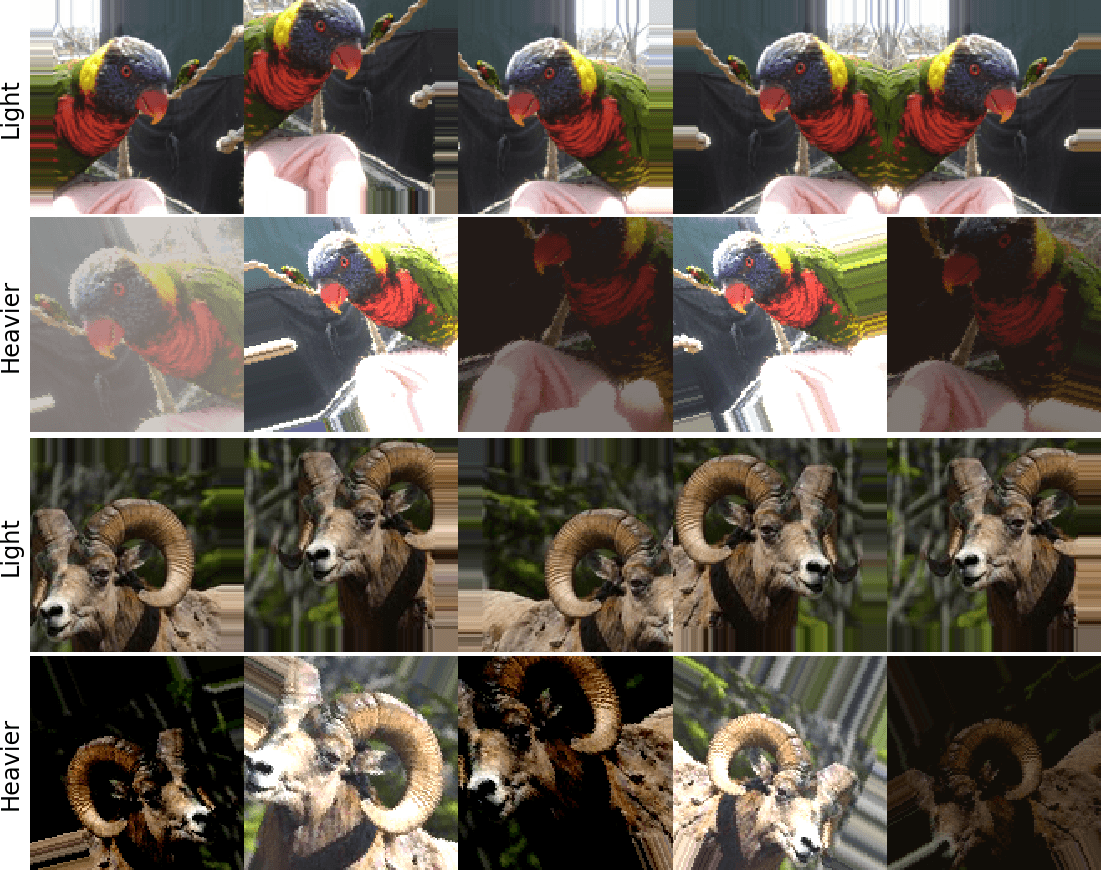
\includegraphics[width = 0.8 \linewidth]{\imgpath/imagenet_daug.png}
  \end{center}
  \caption{Illustration of the transformations performed by the light and heavier augmentation schemes on two example images. Note that the five transformations of the images in this figure have been produced by setting extreme values of the parameters, so as to highlight the characteristics of the schemes and the differences between them.}
  \label{fig:daugit-daugimagenet}
\end{figure}

The performance of All-CNN and WRN trained with light and heavier augmentation is shown in Figure~\ref{fig:daugit-performance}. Note that training with light augmentation provides better results, specially on All-CNN. As pointed out in Chapter~\ref{ch:daugreg}, this is likely explained by first, the fact that the heavier augmentation scheme was not designed to optimise classification, but rather as an arbitrary larger set of plausible transformations; and second, because the limited capacity of the models---especially All-CNN---may prevent them from exploiting the aggressive transformations of the already large ImageNet data set. Nonetheless, the objective of this study was to analyse the learnt representations given a reasonably accurate performance. Ideally, we would also analyse the representations of a model trained with no augmentation. However, the performance without data augmentation is significantly worse and this would likely impact the representations \citep{yamins2014annsbrains}.

\begin{figure}[ht]
  \begin{center}
    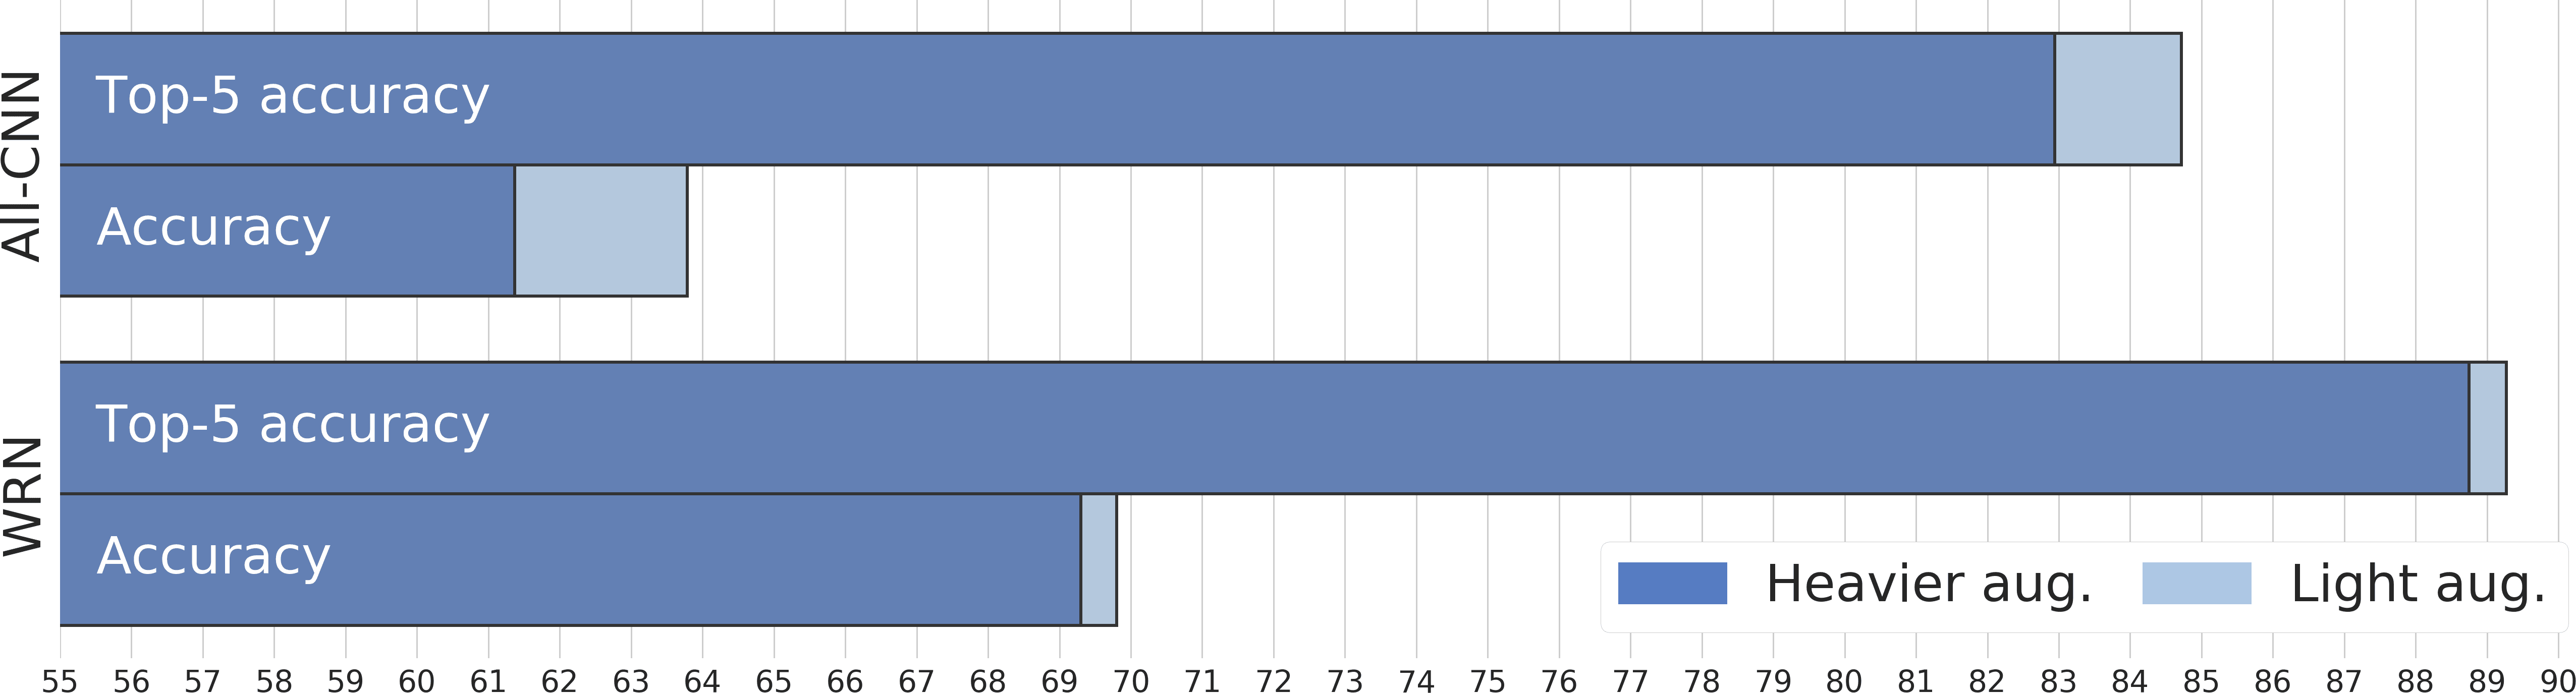
\includegraphics[width = 0.7 \linewidth]{\imgpath/models_performance.png}
  \end{center}
  \caption{Test performance of All-CNN and WRN trained with light and heavier data augmentation.}
  \label{fig:daugit-performance}
\end{figure}

\subsection{Representational similarity analysis}
In order to compare the representations learnt by the neural networks and the activations measured in the inferior temporal cortex, we made use of representational similarity analysis (RSA) \citep{kriegeskorte2008rsa, nili2014rsatoolbox}. The main advantage of RSA is that it allows direct comparisons across different model systems without having to explicitly align the different measurement types. This is accomplished by constructing representational dissimilarity matrices (RDMs) to express the pairwise similarity between stimuli, instead of directly comparing the representations of single stimuli. Across a set of input images, RDMs characterise the internal representations of a given system by storing all pairwise distances. The resulting matrix therefore expresses the representational geometry in the learnt activation space. By relying on distances, RDMs remain unchanged, if the space over which they are computed is rotated.

To characterise the representations in hIT, functional magnetic resonance imaging (fMRI) was used to measure BOLD responses while 15 participants were presented with 92 images of isolated objects. The images originate from a wide variety of categories and levels of abstraction. On the broadest level, they can be separated into animate and inanimate. Inanimate objects can either be natural or artificial, whereas animate objects are divided into human stimuli---heads and body parts---and animals---full body and heads only. This fMRI data set has been used in multiple studies and the details of the data acquisition can be found in \citep{kriegeskorte2008manandmonkey}. In Figure~\ref{fig:daugit-rdms} we show the RDM of the brain data, and the RDMs of the WRN model for illustration. As in \citep{kriegeskorte2008manandmonkey}, in order to better visualise the differences across the RDM, the colour code represents the percentiles of the actual RDMs.

To compare DNNs and hIT representations, the network activation profiles for the 92 images were extracted. In particular, we computed the activations at the outputs of the 12 ReLU layers of All-CNN and at the outputs of the residual blocks of WRN. We then computed the RDM of these activations using the Pearson correlation, as well as the RDM of the fMRI responses in hIT. To obtain a more compact representation of the CNN models, we combined the RDMs of all layers into a single RDM as a linear combination of the individual layer RDMs with respect to the hIT RDM using non-negative least squares and a cross-validation procedure, which avoids overfitting the image set.

\begin{figure}[ht]
  \begin{center}
    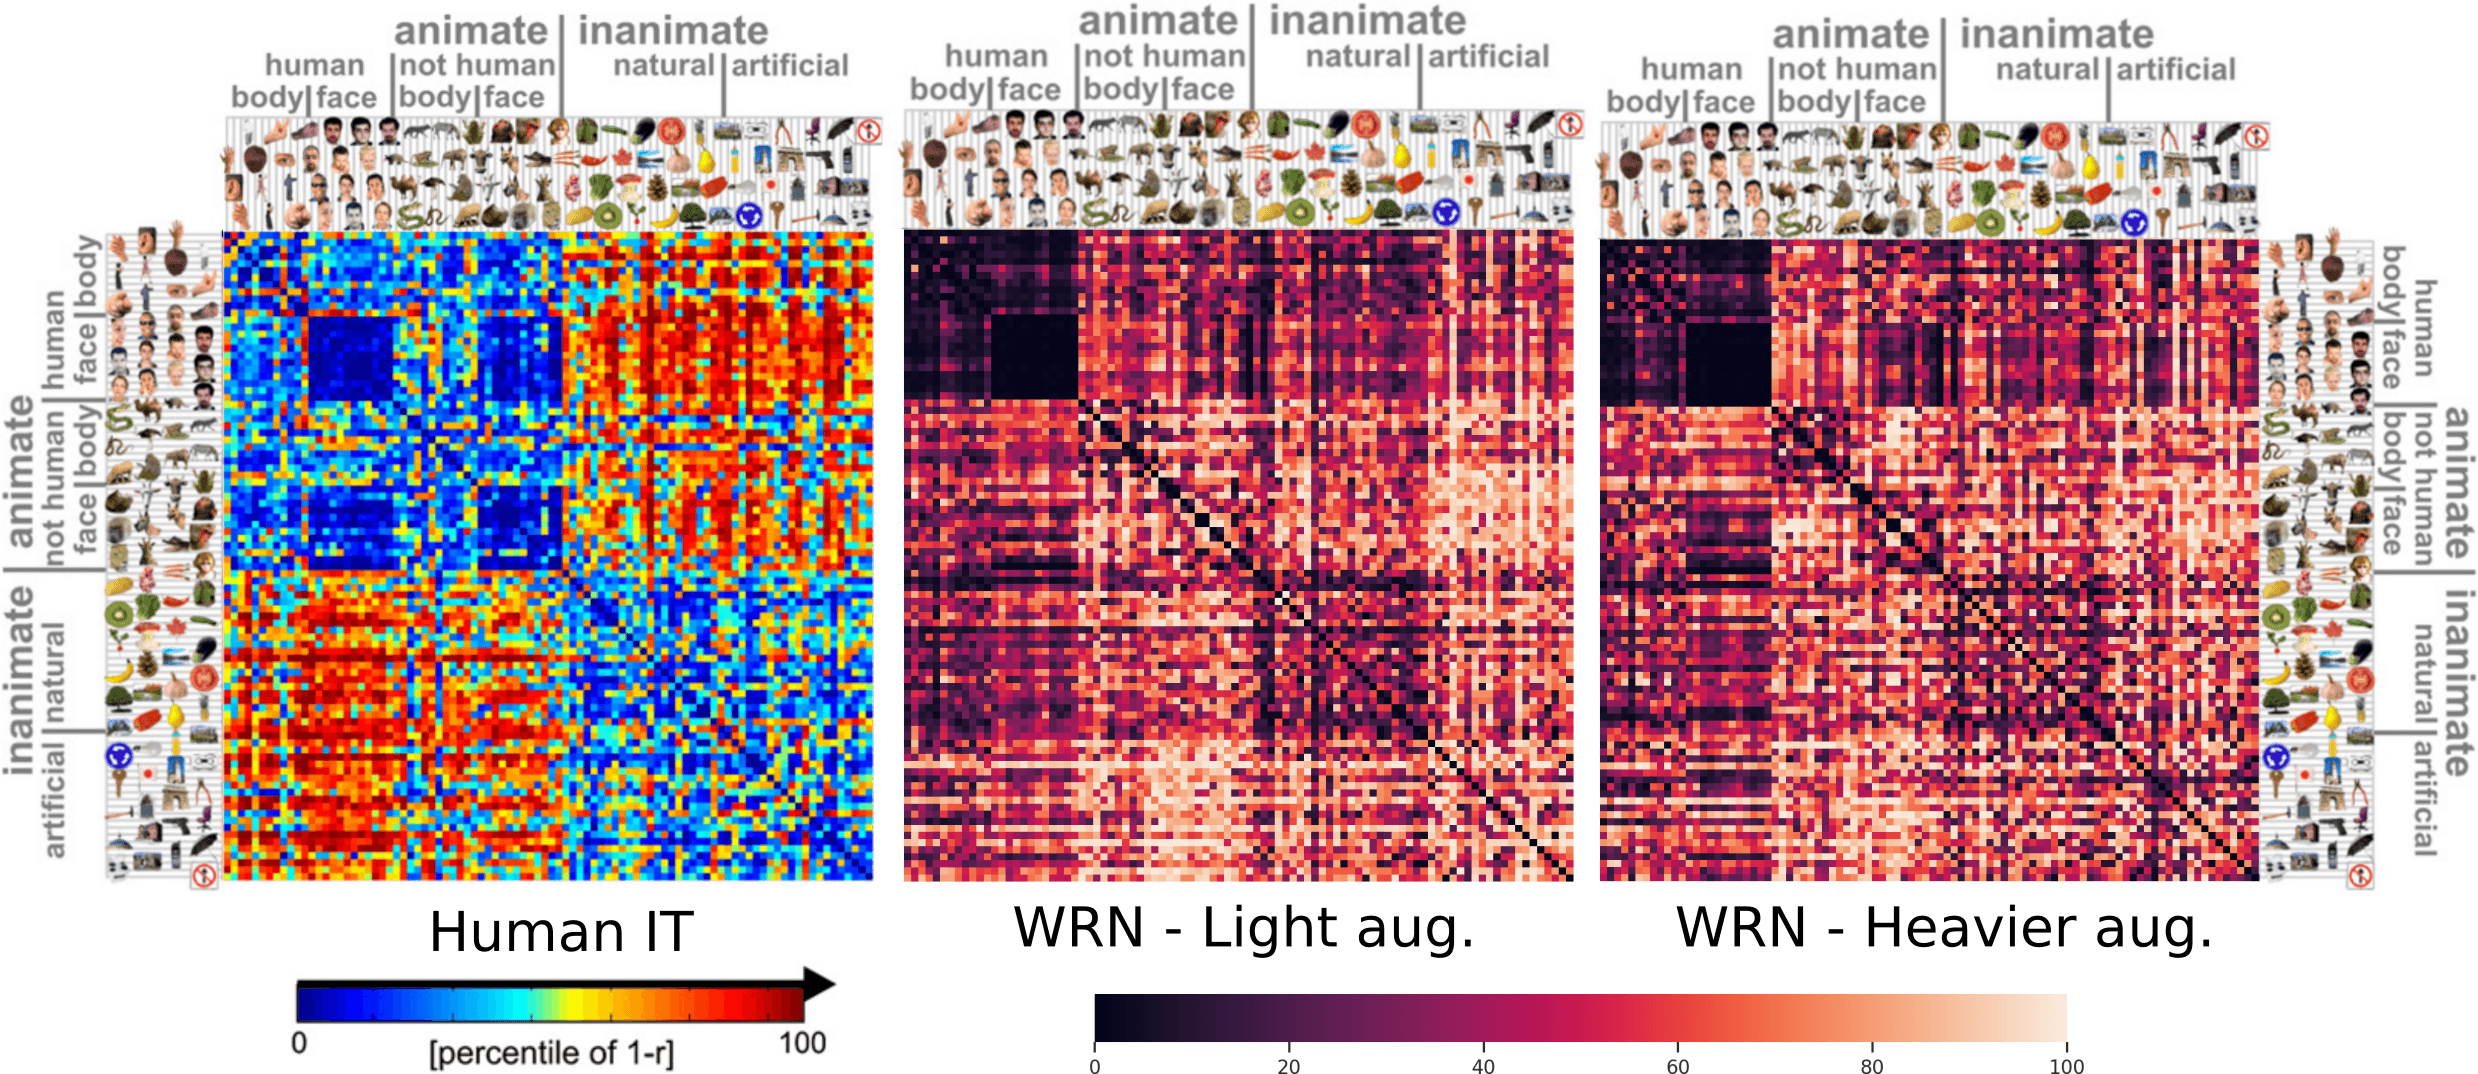
\includegraphics[width = \linewidth]{\imgpath/rdms.png}
  \end{center}
  \caption{RDMs of the systems compared. Left: adapted from \citep{kriegeskorte2008manandmonkey}, the RDM of the human inferior temporal cortex. Centre and right, the RDMs of the WRN model, trained with light and heavier augmentation, respectively. As in \citep{kriegeskorte2008manandmonkey}, the colour code in the matrices shown in the figure represents the percentile of the dissimilarity.}
  \label{fig:daugit-rdms}
\end{figure}

Finally, we characterise the similarity between the artificial neural networks and hIT by computing the Kendall's rank correlation coefficient $\tau_{A}$ between the RDM of the hIT representations and the RDM of the convolutional models. Standard errors were obtained from the similarity estimates of the 15 human subjects.

\section{Results and discussion}
\label{sec:daugit-results}
We show the results of the representational similarity analysis to compare the representations learnt by the neural networks and the fMRI data in Figure~\ref{fig:kendall}. As a main conclusion, we found that the correlation with the hIT representations is significantly higher for the models trained with heavier data augmentation. Not only is this indicated by the Kendall correlation, but also by visual inspection, the RDM of the model trained with heavier augmentations seems more similar to the RDM of the human IT. For example, face images---both human and non-human---form clearer similarity clusters in the model trained with heavier data augmentation, which is a well-studied property of the primate visual cortex. 

In the case of the wide residual network (WRN) the difference between the two levels of augmentation is considerably larger, while in the All-CNN models, although statistically significant ($p<0.05$), the difference is smaller. However, recall that the classification performance of the models trained with heavier augmentations is worse, especially in the case of All-CNN (Figure-~\ref{fig:daugit-performance}. Therefore, it seems that even though the more aggressive transformations do not improve the classification performance, they do increase the similarity with the inferior temporal cortex. 

\begin{figure}[ht]
  \begin{center}
    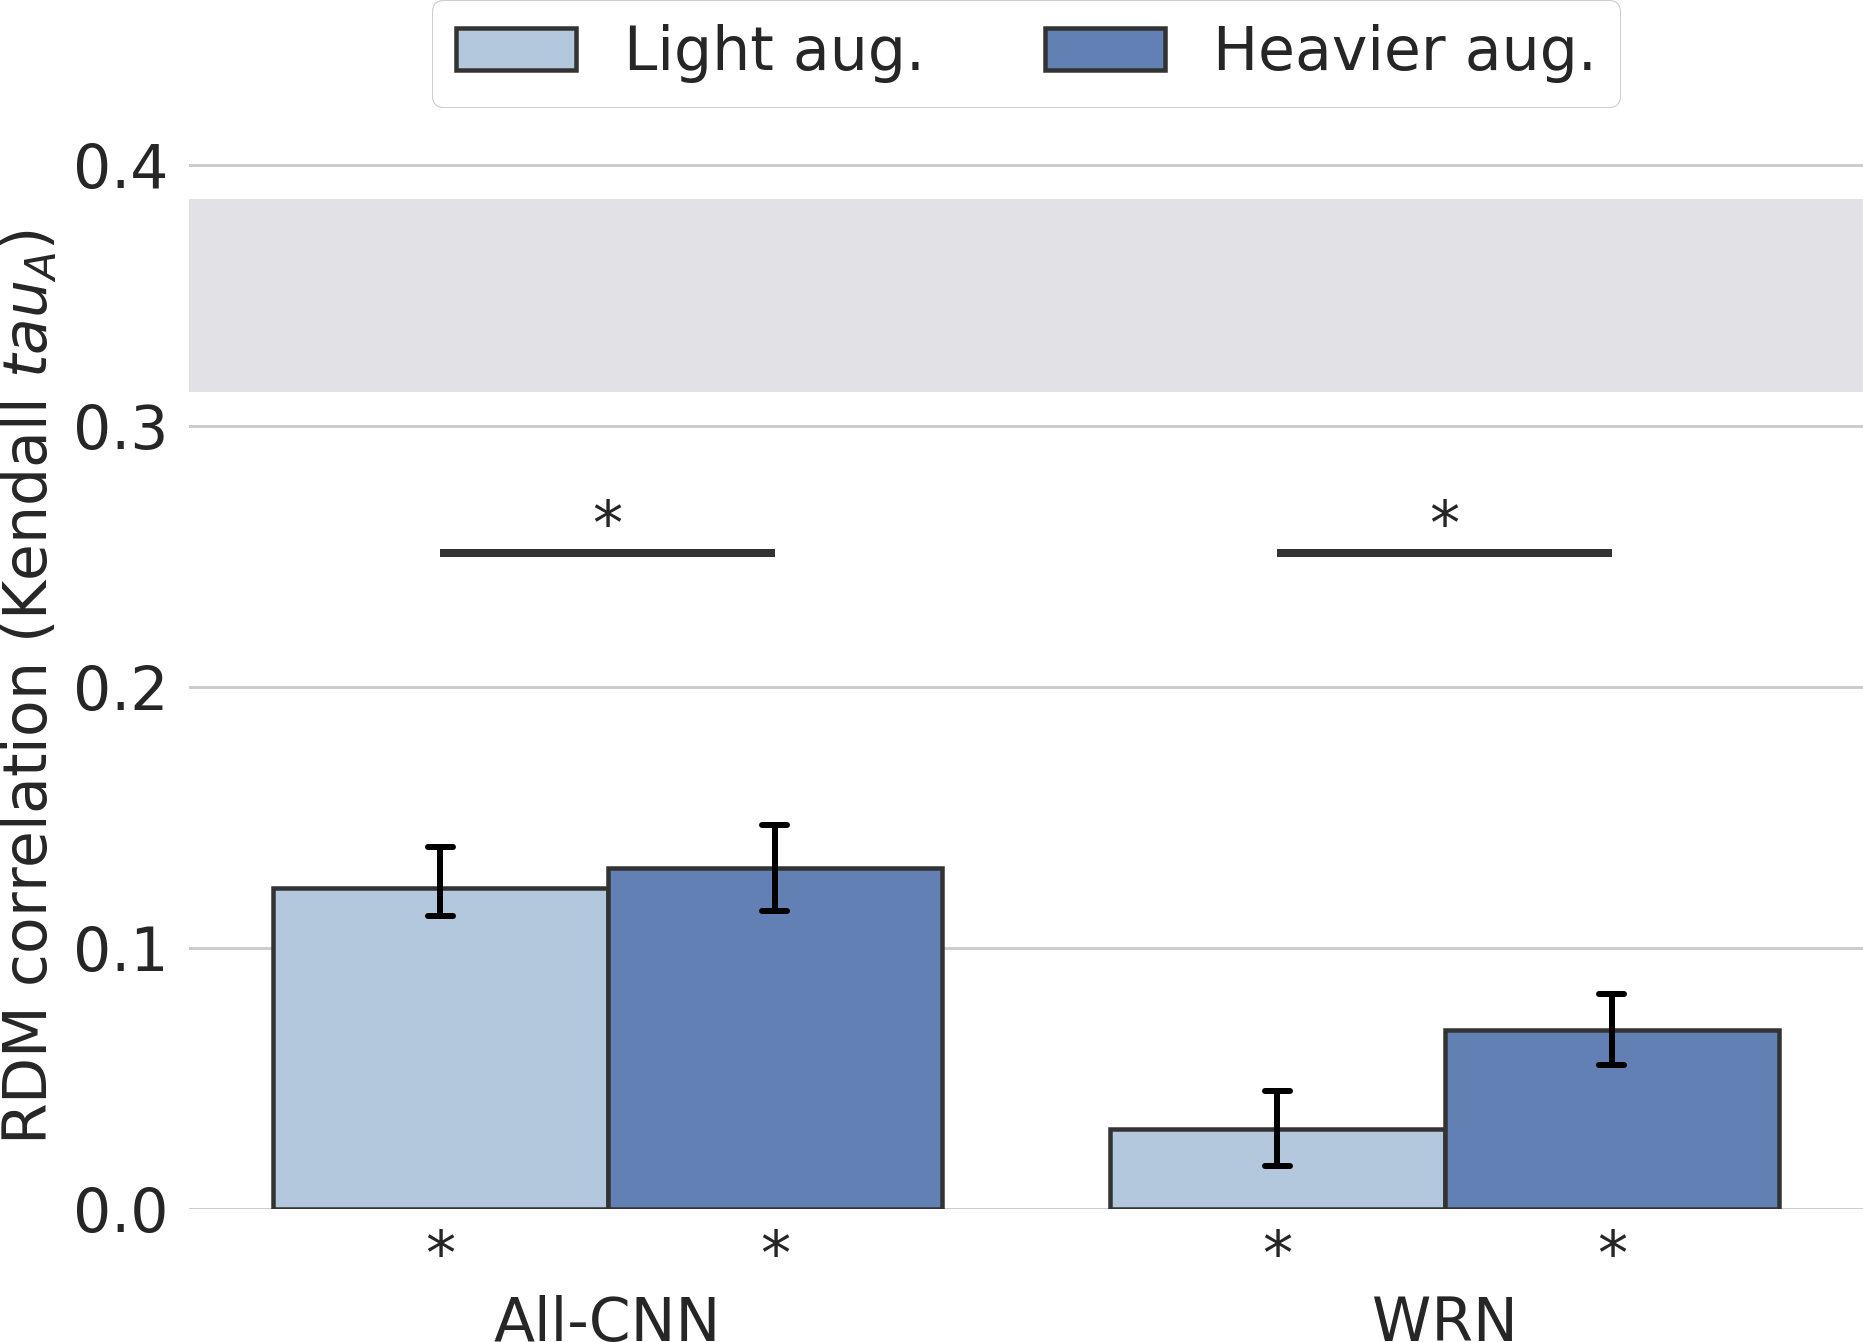
\includegraphics[width = 0.8 \linewidth]{\imgpath/kendall.png}
  \end{center}
  \caption{Comparison of the Kendall's $\tau_{A}$ coefficient of the hIT RDM and the RDM of the networks trained with light and heavier data augmentation. Both on All-CNN and WRN, the correlation of the model trained with heavier transformations is significantly higher than the light counterpart. The grey shaded area indicates the maximum possible correlation of a model given the noise in the measured data.}
  \label{fig:kendall}
\end{figure}

It is also interesting that the similarity with hIT is higher for All-CNN, again despite the lower performance, as opposed to previous work that indicated a correlation between performance and similarity with the visual cortex \citep{yamins2014annsbrains}. The overall lower correlation of WRN adds more evidence to the conclusion of \citet{storrs2017ccn}, who showed that residual networks exhibit a particularly low correlation with hIT compared to other architectures.

Given the exploratory nature of this study, it is not yet clear what exact mechanisms lead to the better match between representational geometries in higher level visual cortex and networks trained with heavier data augmentation. One hypothesis is that the larger variety during training may be more biologically plausible than training with constant images or very light transformations. Humans develop robust object representations based on highly variable input, while freely exploring the world. Sources of variation include different orientations, lighting conditions, backgrounds and occlusion. Eye-movements, including drifts and \textit{microsaccades}, may further contribute to the variability in the sensory input to which the recognition has to be robust. As we will further discuss in Chapter~\ref{ch:invariance}, this robustness is reflected in invariant activations towards identity-preserving transformations in the higher visual cortex.

Our experiments addressed the question as to which factors drive computational models to learn features closer to the brain representations. Given the superiority in visual robustness of the human brain, these insights may have implications for artificial vision systems based on deep neural networks, and for DNNs as a model system for visual processing in the brain. Finding that heavier data transformations leads to more IT-like representations further supports the notion that the input distribution plays a crucial role during the learning of representations in both the brain artificial networks. 

\section{Conclusions}
In this chapter, we have explored how far light and heavier augmentation of the training set can affect the internal representations of deep neural networks and their alignment with human IT. To compare the neural and model system, we used representational similarity analysis, which allows for straightforward comparisons across different modalities---in this case, fMRI BOLD signal and neural network activations. RSA revealed that the neural networks trained with heavier transformations learn representations more similar to those observed in higher visual cortex.

Future work should analyse a larger range of network architectures and data sets to gain better insights into the mechanisms driving the internal representations. It will be also interesting to study the different components of data augmentation in order to understand which particular transformations play a bigger role in better explaining hIT.

\chapterbibliography
}
